%%%%%%%%%%%%%%%%%%%%%%%%%%%%%%%%%%%%%%%%%%%%%%%%%%%%%%%%%%%%%%%%%%%%%%%%%%%
% Copyright (c) 2010 committers of YAKINDU and others.
% All rights reserved. This program and the accompanying materials
% are made available under the terms of the Eclipse Public License v1.0
% which accompanies this distribution, and is available at
% http://www.eclipse.org/legal/epl-v10.html
%
% Contributors:
%     committers of YAKINDU - initial API and implementation
%%%%%%%%%%%%%%%%%%%%%%%%%%%%%%%%%%%%%%%%%%%%%%%%%%%%%%%%%%%%%%%%%%%%%%%%%%%
\documentclass[12pt,ngerman, a4paper]{article}
\usepackage[utf8]{inputenc}
\usepackage{graphicx}
\usepackage{hyperref}
\usepackage{floatflt}
\usepackage{amsmath}
\usepackage{fancyhdr}
\usepackage[top=2cm, bottom=4cm, left=2cm, right=2cm]{geometry} 

%\usepackage{helvet} % Helvetica Schriftart (Arial)

% Setzen des Headers
\setlength{\headwidth}{\textwidth}
\fancyhead[L]{
\includegraphics[height=0.53in]{./Pictures/YakinduLogo}}
\fancyhead[R]{C-Code Generation\\
under ANSI-C and Misra Conformance
}

% Wir wollen eine "Fancy" Ausgabe
\pagestyle{fancy}

% Einstellen einer serifenlosen Schrift
\renewcommand{\familydefault}{\sfdefault}

% Absatzformatierung
\frenchspacing
\parindent 0pt % kein Einrücken bei neuem Absatz
\parskip 8pt    % Abstand zwischen den Absätzen

\begin{document}

% Anpassung des Headers, weil wir hier ja ein Logo drin haben
\setlength\headheight{0.6in}

\tableofcontents

\clearpage
% Dokument startet genau hier
%%%%%%%%%%%%%%%%%%%%%%%%%%%%%%%%%%%%%%%%%%%%%%%%%%%%%%%%%%%%%%%%%%%%%%%%%%%
% Copyright (c) 2010 committers of YAKINDU and others.
% All rights reserved. This program and the accompanying materials
% are made available under the terms of the Eclipse Public License v1.0
% which accompanies this distribution, and is available at
% http://www.eclipse.org/legal/epl-v10.html
%
% Contributors:
%     committers of YAKINDU - initial API and implementation
%%%%%%%%%%%%%%%%%%%%%%%%%%%%%%%%%%%%%%%%%%%%%%%%%%%%%%%%%%%%%%%%%%%%%%%%%%%
\section{Introduction}
In our previous examples we created a YAKINDU state chart with the YAKINDU
Statechart Editor. However, it is also possible to import an existing UML2
state machine or create one with your favourite UML2 tool (You may also use
the UML2 Editor which ships with the eclipse modelling distribution). The tool
of your choice must support "EMF UML2". In our examples we are going to use
the UML2-Toools available in Galileo.

If you want to use an UML2 modelling tool instead of the YAKINDU Statechart
Editor or you have an existing UML2 state machine, you need to consider that
the YAKINDU state charts are somehow different from the UML2 state machines.
To fill this gap you have to extend your UML2 state machine (In future
releases another approach may also be available).

%or, if this is not anoption, you can create extensions for the transformation.

\section{UML2 model}
As for the code genenerators, an example project for transformation of UML2
state machines to YAKINDU state charts is also available. You can open the
examples (see Figure \ref{fig:uml2tools}) and compare them with the generated
YAKINDU state charts. \begin{figure}[ht]
\center
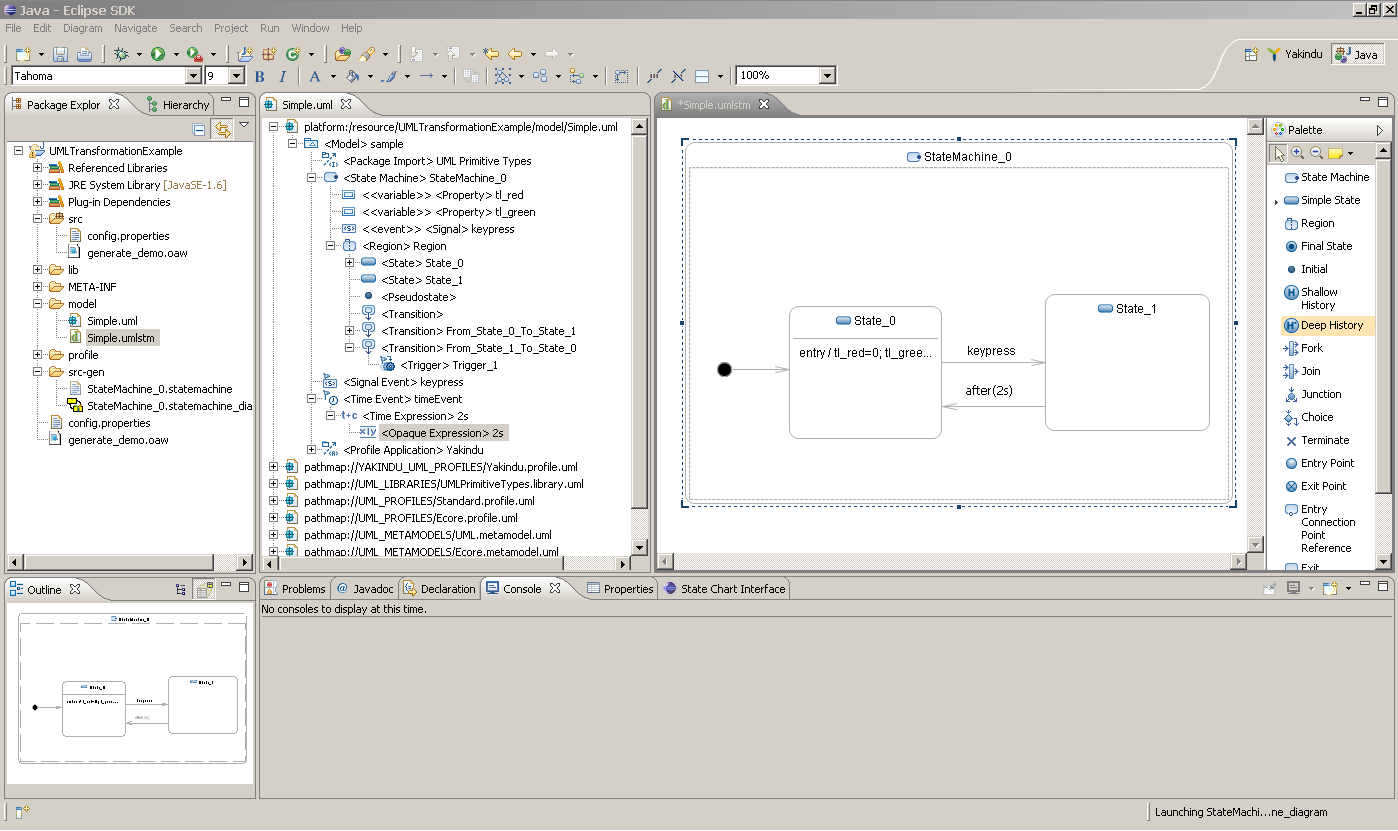
\includegraphics[width=1\textwidth]{Pictures/uml2tools}
\caption{\label{fig:uml2tools}UML2 state machine in eclipse} 
\end{figure}

Some information, which cannot be modelled in UML2 are generated
automatically, or as mentioned before, can be specified somehow else. For
example: Every Transition and every Region in a YAKINDU state chart needs a
priority. On how to set a priority will be discussed later. Lets have a look
at an example project first.

\section{The example project}
The example is available within eclipse under \textbf{File} $\rightarrow$
\textbf{New} $\rightarrow$ \textbf{Example\dots} within the category
\textbf{YAKINDU Examples}. Select ''UML -> YAKINDU Transformation'' and Finish the
dialog. A new project ''UML\_TransformationExample'' containing one UML
diagrams inclusive ''.umlstm'' diagram file for UML tools will be created.

\begin{floatingfigure}[r]{0.3\textwidth}
  \centering
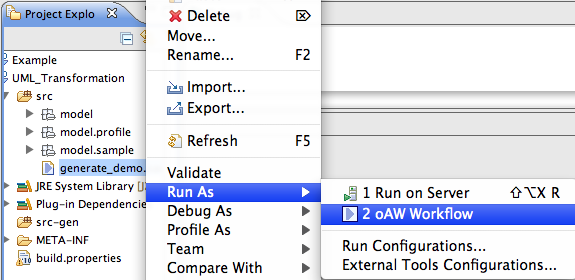
\includegraphics[width=0.3\textwidth]{Pictures/runTransformationUMLAs}
\caption{\label{fig:runTransformationUMLAs}Run UML transformation workflow} 
\end{floatingfigure}
To generate the YAKINDU state chart, right-click on
\textbf{generate\_demo.oaw} and select \textbf{Run As} $\rightarrow$
\textbf{MWE Workflow} (Compare Figure \ref{fig:runTransformationUMLAs}). The
output of the transformation is saved in the new folder src-gen and the status
of the run is available in the Console view of eclipse, which will be
automatically opened in the right corner at the bottom of the window.

The result is a *.statemachine file which can be found in the src-gen folder
within your project. The output folder, where your statemachines will be generated
and the UML2 model can be defined in the generatordemo.oaw. The next step,
which should follow, is to generate a diagram for your model. This is not
automatically done, but with a right-click on the statemachine file you can
initialize a diagram (see figure \ref{fig:initializeDiagram}). Because the
layout information are not stored inside UML2 you have to draft your diagram
by hand. \begin{figure}[ht]
\center
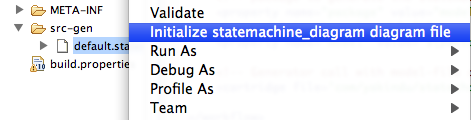
\includegraphics[width=0.6\textwidth]{Pictures/initializeDiagram}
\caption{\label{fig:initializeDiagram}Initialize Diagram} 
\end{figure}

The generated state chart can be edited, simulated and code can be generated
from it. These steps were described in previous chapters. If you want to
generate code from the state chart see Chapter \ref{sec:CCodeGenerator} for C
and Chapter \ref{sec:JavaCodeGenerator} for Java. If the model is a valid
YAKINDU state chart a simulation is also possible (see Chapter
\ref{sec:simulatingStateMachine}).

\section{How does it work}
The UML2 state machine and the YAKINDU state chart are quite similar.
Nevertheless, there are a few differences that need to be cared of.

\subsection{Name mapping}
The naming is the smallest gap. The following table shows the name mapping
between the UML2 state machine and the YAKINDU state chart.

\begin{table}[ht]
\begin{center}
\begin{tabular}{|c|c|}
\hline UML2 & YAKINDU \\
\hline
StateMachine & Statechart \\
Region & Region \\
Transition & Transition \\
Vertex & Node \\
State &  State \\
FinalState & FinalState \\
Pseudostate & Pseudostate \\
\hline
\end{tabular}
\end{center}
\caption{UML2 - YAKINDU Mapping}
\label{UML2 - YAKINDU Mapping}
\end{table}

As you can see, there are only marginal differences. Besides that, YAKINDU state
chart also defines new elements which are not present in the UML2.

\subsection{New elements}
The new elements are Variable and Event. As those can't be mapped 1:1, some
conventions are needed. The default behavior of the transformation is to ignore
those elements. This will result in an incomplete YAKINDU state chart (therefore
no simulation is possible). To %prevent this, you can decide between two methods.
prevent this, you have to extend your UML2 state machine.

\subsection{Limitations}
There are a few UML Elements that are currently not supported by the transformation. That includes the
PseudoStates
\begin{itemize}
\item join
\item fork
\item entryPoint
\item exitPoint
\item and terminate.
\end{itemize}
A transformation that encounters such
an element will fail.

\subsection{Transformation Cartridge}
The Transformation Cartridge allows you to integrate the YAKINDU Transformation into
your oAW Workflow. The cartridge expects the following parameters.

\begin{table}[ht]
\begin{center}
\begin{tabular}{|l|l|}
\hline Parameter & Description \\
\hline
umlModel & A path to your UML2 Model file. \\
srcgen &  The output folder where the generated *.statemachine files should be created. \\
package &  The root directory for the transformation. \\
\hline
\end{tabular}
\end{center}
\caption{YAKINDU Transformation Cartridge Parameters}
\label{YAKINDU Transformation Cartridge Parameters}
\end{table}

In your oAW Workflow it may look like this:\begin{verbatim}
...
<property name="umlModel" value="model/Simple.uml"/>
<property name="src-gen" value="src-gen"/>
<property name="config" value="src/" />

<!-- Generator call with model-file and output-folder -->
<cartridge file='com/yakindu/statechart/transformation/uml2/transform.oaw' 
	project="com.yakindu.statechart.transformation.examples.uml2"
 	umlModel="${umlModel}" 
 	src-gen="${src-gen}" 
 	config="${config}" />
...
\end{verbatim} 


\section{Extending an UML2 state machine}
% The first method is to modify your UML2 state machine.
Since there aren't UML2 Elements called Variable or Event, those have to be
created with the existing UML2 elements and the YAKINDU UML2 profile. The profile
allows you to give Transitions and Regions a priority and to describe Events as
Signals and Variables as Classes.

First you need to apply the YAKINDU UML2 profile.  Open your *.uml file and select the model.
Click on \textbf{UML Editor} $\rightarrow$ \textbf{Package} $\rightarrow$
\textbf{Apply Profile}. A new window pops up where you add the YAKINDU UML2
profile to your model. Press \textbf{Ok} and save the *.uml file. Now that the
profile has been loaded you need to apply the stereotypes to various elements.
You can do this with the UML Editor which has been used until now.
\begin{figure}[h!]
\center
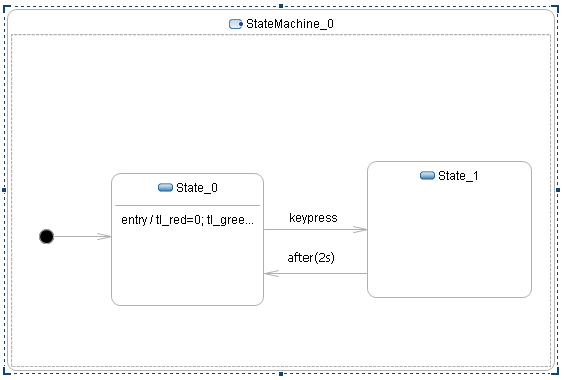
\includegraphics[width=0.5\textwidth]{Pictures/priorityVisualisation}
\caption{\label{fig:priorityVisualisation}UML2 state machine example} 
\end{figure}

Open the related *.umlstm file. It should look somehow like Figure
\ref{fig:priorityVisualisation}. The YAKINDU UML2 profile allows us to apply the
stereotypes Priority, Variable and Event. Priority can be applied to Transitions
and Regions, Variable to Classes and Event to Signals. First, we want to give
every Transition and every Region a Priority. To do so, select a
Transition/Region in the UML Editor. Select \textbf{UML Editor} $\rightarrow$ \textbf{Element} $\rightarrow$
\textbf{Apply Stereotype\dots}. Afterwards you can edit the priority in the properties tab, if element is selected.
\begin{figure}[h!] \center
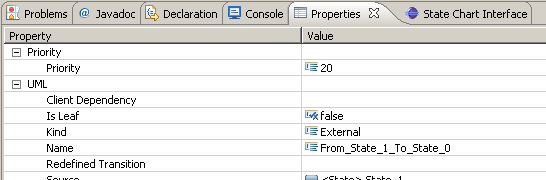
\includegraphics[width=0.9\textwidth]{Pictures/changePriority}
\caption{\label{fig:changePriority}Change the Priority} 
\end{figure}
The default value for Priority is 0 (see figure
\ref{fig:changePriority}). That's it! Repeat this for every Transition/Region in
your State machine.

Now we are going to add the Stereotypes Event to our Signals. Most work will be done in the tree UML Editor. 
\begin{figure}[h] \center
\includegraphics[width=0.9\textwidth]{Pictures/editorApplyStereotype}
\caption{\label{fig:editorApplyStereotype}Apply Stereotype} 
\end{figure}

Select a Signal and click on \textbf{UML Editor} $\rightarrow$ \textbf{Element}
$\rightarrow$\textbf{Apply Stereotype} (see figure
\ref{fig:editorApplyStereotype}). Add YAKINDU::Event and press \textbf{OK}. In
the Properties View you can see now a Property Event with some Attributes.
\begin{figure}[h] 
\center
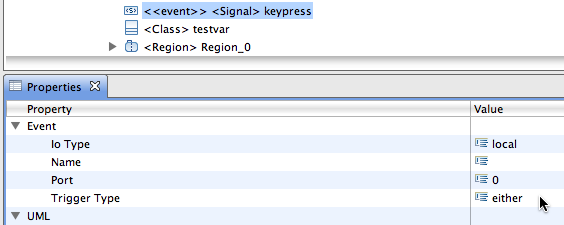
\includegraphics[width=0.9\textwidth]{Pictures/editorProperty}
\caption{\label{fig:editorProperty}Change Attributes} 
\end{figure}
Change those Attributes to your needs (see figure \ref{fig:editorProperty}).
Repeat this for every Signal in your state machine.

To add Variables to your UML2 state machine you have to create properties for your variable first. 
\begin{figure}[h] 
\center
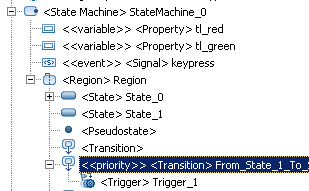
\includegraphics[width=0.7\textwidth]{Pictures/variableExpression}
\caption{\label{fig:variableExpression}Property named after a Variable} 
\end{figure}

Those have to be named after the Variables in the Expressions of your Transitions
(see figure \ref{fig:variableExpression}). If you created a Property, select it and click
on \textbf{UML Editor} $\rightarrow$ \textbf{Element} $\rightarrow$
\textbf{Apply Stereotype}. Add YAKINDU::Variable and press \textbf{OK}. In the
Properties View you can change now the Attributes of Variable to your needs.
Repeat this for every Variable in you Expressions.

It is important to know that Signals and Properties that should be recognized as Events
and Variables must be created under the state machine in the UML2 model. This is
necessary due to the fact that any number of state machines can be in a UML2 model.

If you followed all the described steps you are now able to generate a valid
YAKINDU state chart.


%(ok)- how to use the transformation by example
%- how to simulate a transformed model
%(code?)- how to generate from a transformed model
%- how the transformation works (important mapping rules)
%-> Role of clasifier/class
%-> (done) using the profile
%-> (not yet) using alternatives to the profile


\clearpage
%%%%%%%%%%%%%%%%%%%%%%%%%%%%%%%%%%%%%%%%%%%%%%%%%%%%%%%%%%%%%%%%%%%%%%%%%%%
% Copyright (c) 2010 committers of YAKINDU and others.
% All rights reserved. This program and the accompanying materials
% are made available under the terms of the Eclipse Public License v1.0
% which accompanies this distribution, and is available at
% http://www.eclipse.org/legal/epl-v10.html
%
% Contributors:
%     committers of YAKINDU - initial API and implementation
%%%%%%%%%%%%%%%%%%%%%%%%%%%%%%%%%%%%%%%%%%%%%%%%%%%%%%%%%%%%%%%%%%%%%%%%%%%
\section{Example Scenario}

The example scenario is a simple pedestrian traffic light. A pedestrian can press
a button to indicate, she/he wants to cross the street. Then a blinking white
light indicates, that the traffic light has recognized the request. After a few
seconds, the traffic light for the street turns to red and the pedestrian traffic
light turns to green. Then the pedestrian traffic light turns to red and the
street traffic light changes to green again.
    
The state machine to model this behaviour is shown on figure
\ref{fig:statemachine}. This state machine must not be created but is shipped
with the example project and can be found in the
\texttt{workspace/Traffic\_Light/} directory.
    
\begin{figure}[ht] \center
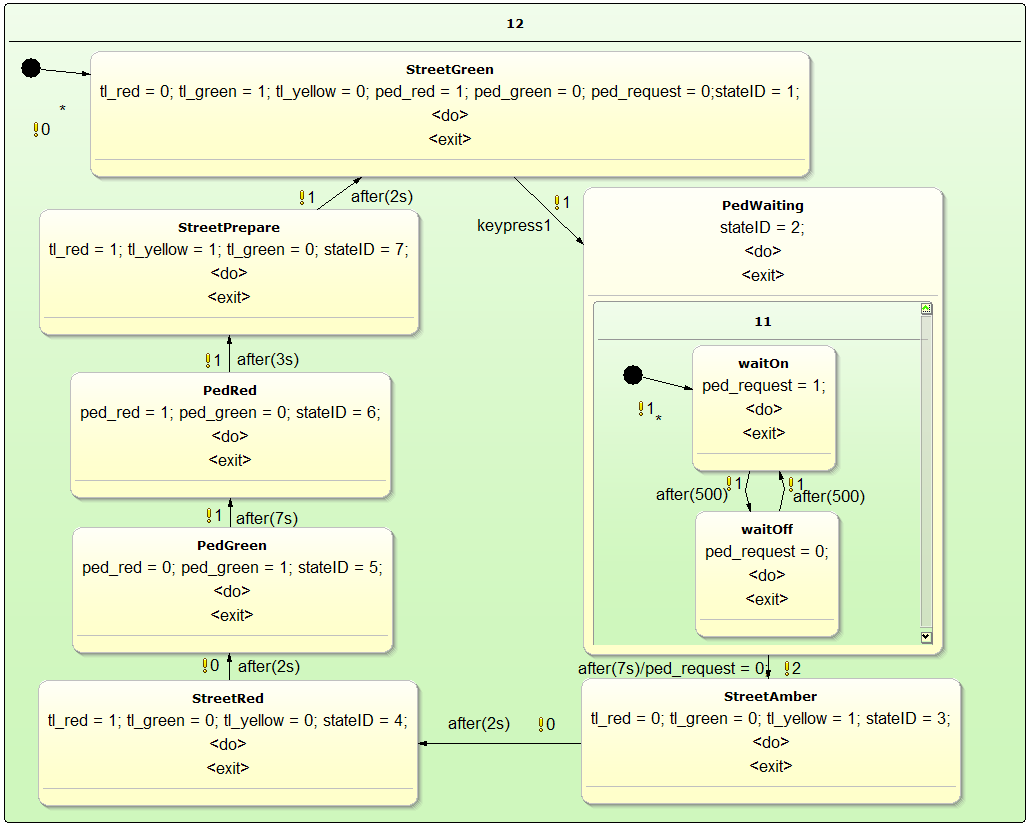
\includegraphics[width=0.8\textwidth]{./Pictures/Statemachine}
\caption{\label{fig:statemachine}Statemachine for the Traffic Light Example}
\end{figure}

% The embedded system that is used with this scenario is a ATMega128 Controller
% on a Display3000 board. This system was extended by an additional board
% representing a traffic light controlled crossroad. This board is connected to
% the Display3000 board.

\section{Starting the workflow}

The source code is created by starting the MWE workflow. This workflow can be
found in the \textit{traffic light} example directory:

\begin{figure}[h!] \center
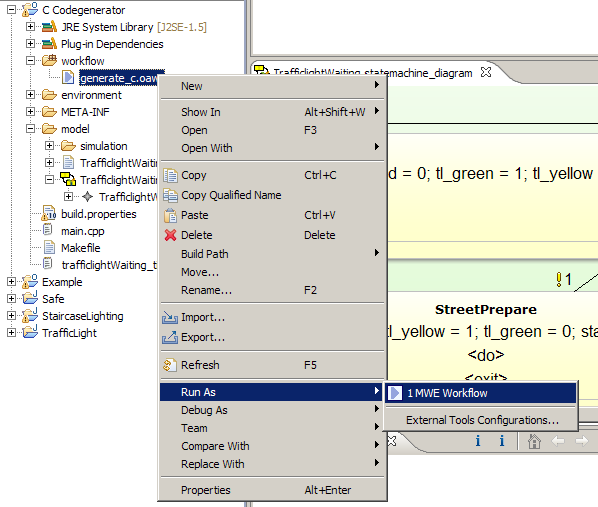
\includegraphics[width=0.8\textwidth]{./Pictures/workflow}
\caption{\label{fig:workflow}Starting the oAW-workflow to create the sources}
\end{figure}
\newpage

The generated C source code can be found within the new directory \texttt{c-src-gen}:

\begin{figure}[h!] \center
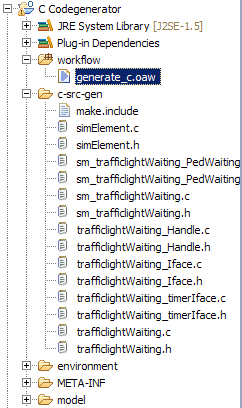
\includegraphics[width=0.3\textwidth]{./Pictures/sources}
\caption{\label{fig:sources}The sources are placed into the \textit{c-src-gen} directory}
\end{figure}

\newpage
%Hier fehlt noch was: wie wird der Workflow gestartet, und was muss alles vorhanden sein, damit der workflow tatsaechlich starten kann.
%-> Nutzer oAW
%-> Wo liegt das Ergebnis (Code)
%-> was kann man einstellen (Properties)

\section{Code Integration into an Existing Project}

Aside the source code for the state machine and the code for the interfaces, the
code generator creates a file called \texttt{make.include}. This file can easily
be included into an existing makefile by the line:

\begin{verbatim}
include c-src-gen/make.include
\end{verbatim}

The files, which are needed for the compilation, are added to the environment
variable \texttt{SM\_SOURCE}, so you have to add these sources to your project
sources:

\begin{verbatim}
OBJECTS    = main.o $(ENV_OBJ) $(GRAPHIC_OBJ) $(SM_SOURCE)
\end{verbatim}
%$

Additionally you should add the \texttt{c-src-gen} directory to the include and
source paths, so that the headers and sources could be found.
 
The example is designed for the Display3000 board, so the \textbf{Makefile} was
designed to create a binary for this hardware. Therefor it requires the AVR-gcc
toolchain to be able to compile. The toolchain contains a compiler, a linker and
some other usefull tools e.g. to download the data.

So go to your workspace directory with a shell and from there into the base
directory of your project and call \texttt{make}:

\begin{verbatim}
workspace$ cd Traffic_Light
Traffic_Light$ make
[...] compiling [...]
avr-gcc -Wall -Os -DF_CPU=7456000 -mmcu=atmega128 -I. -I./graphicLib [...]
rm -f main.hex
avr-objcopy -j .text -j .data -O ihex main.elf main.hex
\end{verbatim} 

If the compile was successful, you have a working binary \texttt{main.hex} that
could be deployed on the target.

To transfer the binary, you can use \texttt{make flash}.

\section{State Machine Access}

As mentioned before, the code for the state machine can be found in the folder
\textbf{c-src-gen}. After running the workflow the following files should be
available in this directory:

\begin{verbatim}
c-src-gen$ ls
make.include                        sm_trafficlightWaiting_PedWaiting.h
simElement.c                        trafficlightWaiting.c
simElement.h                        trafficlightWaiting.h
sm_trafficlightWaiting.c            trafficlightWaiting_Iface.c
sm_trafficlightWaiting.h            trafficlightWaiting_Iface.h
sm_trafficlightWaiting_Handle.c     trafficlightWaiting_timerIface.c
sm_trafficlightWaiting_Handle.h     trafficlightWaiting_timerIface.h
sm_trafficlightWaiting_PedWaiting.c
\end{verbatim}
% $

The files completely define the state machine. How to integrate the source into
another project, was subject of the previous section.

The files \texttt{sm\_trafficlightWaiting.*} and
\texttt{sm\_trafficlightWaiting\_PedWaiting.*} represents the two regions in the
state chart. The header- and C-file called
\texttt{sm\_trafficlightWaiting\_Handle.*} contain the main handle, which is
called \texttt{SM\_trafficlightWaiting\_Handle}. Please do not access the state
machine handle information directly.

The structure carries the information about the current state, the actual
transition, that has been activated, the handle for the first level region and
the interface handle. The handle is initialized with the function
\texttt{trafficlightWaiting\_init(\&sMachineHandle, \&interfaceHandle)}. Here the
\texttt{sMachineHandle} is the state machine handle and the
\texttt{interfaceHandle} is a \underline{pointer} to an interface handle. The
initialization call initializes the whole state machine and returns the interface
handle pointer.

For convenience all a state machine user needs to include is
\texttt{trafficlightWaiting.h}. This header includes all other necessary
information.
 
\section{Operating System and Drivers for the Example Device}

To let the state machine run on the Display 3000 development board, the system
needs a minimal \textbf{operating system} (OS) and some drivers for input and
output. This operating system is found in the \texttt{environment} directory.
This cooperative OS is written in C++ and contains an input driver for the 6 keys
on the hardware board and an output driver for the display and a LED board that
is connected to the \textit{port A}.

Because of copyright restrictions, the display driver is not included into this
example. The calls to the display interface can included by adding
\texttt{-DWITH\_DP3000\_GL} to the compiler options and updating the include
path defined in variable \texttt{COMPILETT} of the Makefile to point to the
right AVR-Libraries.

The transfer of the LED data uses a simple software driven SPI-like interface
with three connections (data, clock and inherit).

The rest, like shifting the data, is done by the hardware board.

Following files belong to the operating system:
\begin{verbatim}
definitions.h  event.h      scheduler.cpp  task.cpp
event.cpp      prioQueue.h  scheduler.h    task.h
\end{verbatim}

The \texttt{key*} files contain the driver for a debounced key input. The
\texttt{output*} files contain the driver code to create the output. To create
the cycles for the state machine, this behaviour is placed in the files
\texttt{statemachine*}.

\begin{figure}[h!]
\center
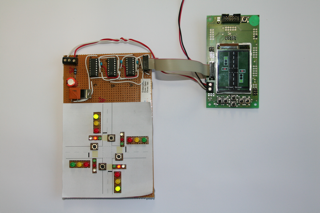
\includegraphics[width=0.8\textwidth]{./Pictures/Board1}
\caption{\label{fig:board1}Display3000 Development board with additional Hardware}
\end{figure}

After generation of source code by the workflow, it is possible to call the
Makefile inside the root directory of this example. By default this File calls
the commands \textbf{avr-gcc} and \textbf{avr-g++}. If you like to send
the binary to the micro controller, it is neccessary to check the \texttt{PORT}
variable inside the Makefile and \textbf{avrdude} needs to be on classpath. If
everything is correct, \texttt{make flash} will send the binary to the controller.
\newpage


%%%%%%%%%%%%%%%%%%%%%%%%%%%%%%%%%%%%%%%%%%%%%%%%%%%%%%%%%%%%%%%%%%%%%%%%%%%
% Copyright (c) 2010 committers of YAKINDU and others.
% All rights reserved. This program and the accompanying materials
% are made available under the terms of the Eclipse Public License v1.0
% which accompanies this distribution, and is available at
% http://www.eclipse.org/legal/epl-v10.html
%
% Contributors:
%     committers of YAKINDU - initial API and implementation
%%%%%%%%%%%%%%%%%%%%%%%%%%%%%%%%%%%%%%%%%%%%%%%%%%%%%%%%%%%%%%%%%%%%%%%%%%%
\section{Detailed usage information}

\subsection{Regions}
\label{sec:Regions}

A region is a sub-state machine that runs concurrently to the other regions. To
serialize the processing of the sub-state machines within the regions, the
regions possess a priority. The region with the highest priority is processed
first.

\begin{figure}[ht] \center
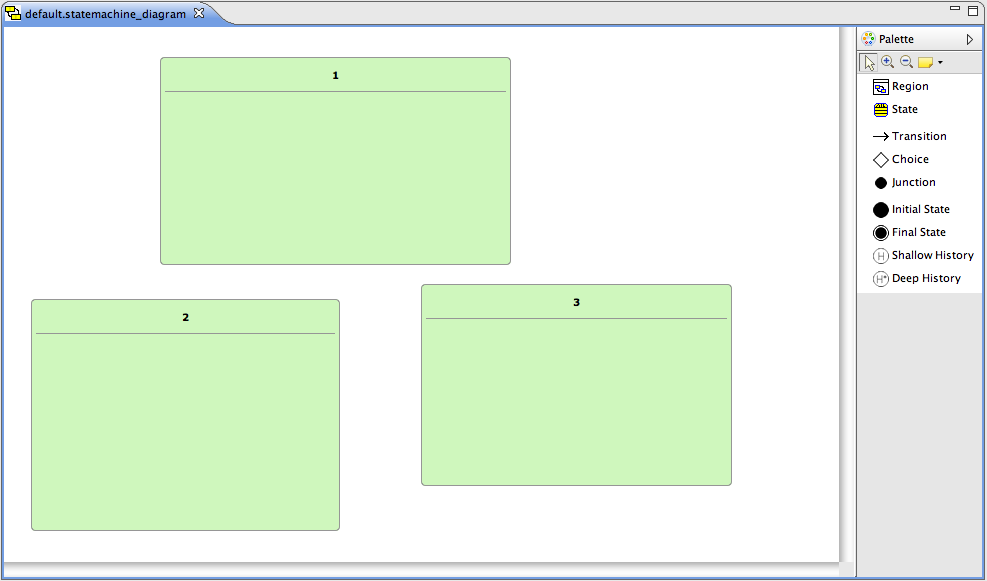
\includegraphics[width=0.7\textwidth]{./Pictures/RegionsPlain}
\caption{\label{fig:RegionsPlain}Three regions within a State Machine Diagram.}
\end{figure}

In the actual YAKINDU version, the regions are not hierarchically aggregatable.
  
\subsection{States}
\label{sec:States}

The states are the main elements of a state machine as they specify the possible
states the state machine consist of. Every state has a unique name, which must be
set by the user.

\begin{figure}[ht]
\center
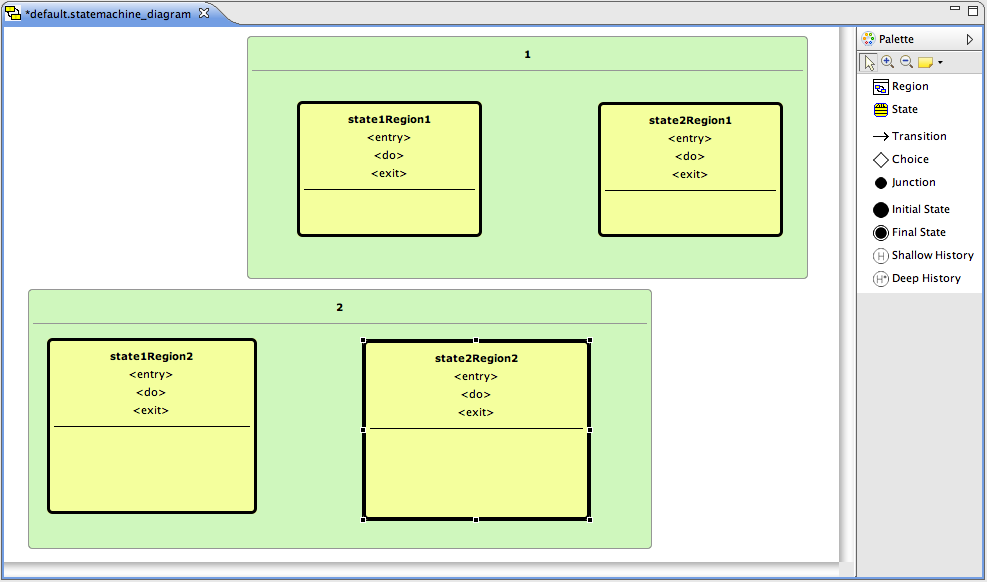
\includegraphics[width=0.7\textwidth]{./Pictures/statesInRegions}
\caption{\label{fig:statesInRegions}Two regions with two states each}
\end{figure}

The parameters of this state are:

\begin{itemize}
\item \textbf{Entry:} The actions, which are performed on the arrival in this
state are specified in the $<entry>$ area. 
\item \textbf{Do:} The actions, which are performed while the state does not 
change, is specified in the $<do>$ area.
\item \textbf{Exit:} The actions, which are performed when a status is left, is
specified in the $<exit>$ area.
\end{itemize}

%Hier fehlt noch: wie genau ist die "expression" die hier einzutragen ist definiert.
 
\newpage 

\subsection{Pseudostates}
\label{sec:Pseudostates}

Pseudostates are states, that do not have any $<entry>$, $<do>$ or $<exit>$
areas. These states are used to specify special states like the \textbf{Initial
State} or the \textbf{Final State}.

Actually the following states are defined:

\begin{itemize}
\item \textbf{Initial State:} The \textbf{Initial State} is the state where the
state machine or the sub-state machine specified by a region start with. Usually
the \textbf{Initial State} is connected unconditionally with another normal
state. 
\item \textbf{Final State:} The \textbf{Final State} is the state where a
state machine ends. When the \textbf{Final State} is reached, the state machine
usually stops processing. 
\item \textbf{Shallow History:} The \textbf{Shallow
History} carries the last active state within a sub-state machine. When this
sub-state machine is re-entered, the last active state is set active again. 
\item \textbf{Deep History:} The \textbf{Deep History} works as the \textbf{Shallow
History} but can also handle nested sub-state machines, so that the correct
nested sub-state machine is used when a sub-state machine is entered. 
\item \textbf{Choice:} A \textbf{Choice} a an element to branch a transition. Every
branch of a transition must have it's own transition condition. An example is a
transition, that is started with a trigger signal and then splits up to arrive at
state X or state Y depending on a guard variable. 
\item \textbf{Junction:} The
\textbf{Junction} connects two transitions that have the same target state.
\end{itemize}

\subsection{Transitions}
\label{sec:Transitions}

\textbf{Transitions} specify the change from one state to another. Every
\textbf{Transition} must have a condition on which the state switch takes place.
The syntax for this condition is:

\begin{verbatim}
Trigger1, Trigger2, \dots, TriggerN[Guard]/Action1; Action2; \dots ActionM; 
\end{verbatim}

\begin{itemize}
\item \textbf{Trigger:} A trigger is activated by an outside event. If more than
one trigger is specified all triggers are connected by \textbf{OR}.

A special trigger is specified by the \textit{after($<duration>$)} keyword. This
keyword defines a duration after which a transition is performed. The
$<duration>$ is an integer number with a specifier (e.g. $after(12s)$).

\item \textbf{Guard:}  A guard is a boolean expression. Example: \texttt{A==B}
\item \textbf{Action:} An action consists of instructions, that should be
performed during transition. This action should be short to have a reliable flow.
\end{itemize}

Additionally every \textbf{Transition} needs a unique priority. The reason is
that every \textbf{Transition} have to be unique, so that the state machine
always behalves in the same way independent of the sequence the
\textbf{Transitions} are created for example.

\subsection{Variables and Events}

The state machine is driven only by triggers and guarded variables, as discussed
in section \ref{sec:Transitions}. These two types of variable data can only be
used within a transition expression, if the variables and events (which results
in triggers) are defined.

To define a variable or an event, you open the \textbf{State Chart Interface} and
right-click on either \textbf{Events} or \textbf{Variables}.

The dialog \textbf{Create Variable} requests at least a name for the variable.
Additionally, the variable can have a \textbf{Port}. The \textbf{I/O-type}
specifies whether the variable is a local, input or output variable. At last, the
\textbf{Data Type} can be chosen between integer (int), floating point (double)
or boolean (bool).

Events are very similar to variables. The main difference during event creation
is that you can not specify a \textbf{Data Type} but a \textbf{Trigger Type}
which can hold the values \textit{raising}, \textit{falling} or \textit{either}.

\subsection{Interfaces}

To interact with the state machine the system designer can add interface
functions within an actions expression. These functions must follow the
\textbf{Action Function Pointer} definition (i.e. the function is returning void
and does not have any parameter). To meet the MISRA requirements, a function
pointer must be a constant pointer, which means that the interface function must
be bound to the state machine during compile time. So there is no late binding
available in this case.


\end{document}

